\usetikzlibrary{shapes.geometric}

\begin{frame}{exceptions [Venn diagram]}
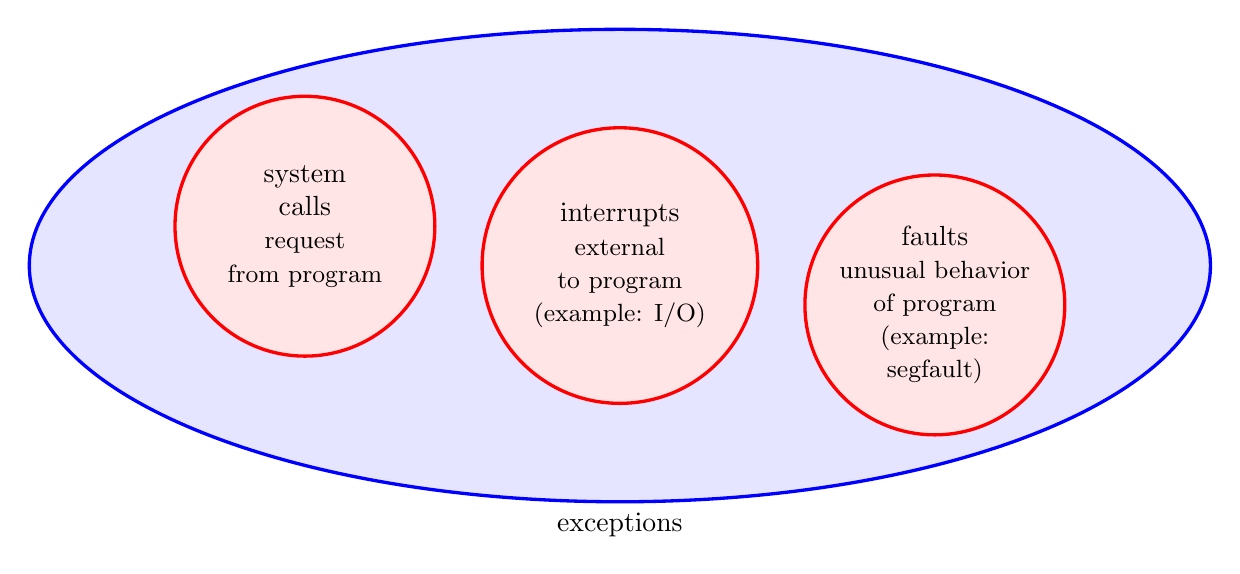
\begin{tikzpicture}
\node[very thick,draw,ellipse,blue,fill=blue!10,label={south:exceptions},minimum width=15cm,minimum height=6cm] (except) {};
\node[very thick,draw,circle,red,fill=red!10,label={[align=center]center:system\\calls \\\small request \\\small from program},
      minimum width=3.3cm] (syscalls)
    at ([xshift=-4cm,yshift=.5cm]except.center){};
\node[very thick,draw,circle,red,fill=red!10,label={[align=center]center:faults\\\small unusual behavior \\\small of program\\\small(example:\\\small segfault)},
      minimum width=3.3cm] (fault)
    at ([xshift=4cm,yshift=-.5cm]except.center){};
\node[very thick,draw,circle,red,fill=red!10,label={[align=center]center:interrupts\\\small external\\\small to program\\\small (example: I/O)},
      minimum width=3.5cm] (intr)
    at ([xshift=0cm,yshift=0cm]except.center){};
\end{tikzpicture}
\end{frame}
